\subsection{Autoregressive integrated moving average}

Based on the hypothesis that the \texttt{daily count of transactions} for a given customer for a certain point in time is correlated to some lagged values before that point in time, a model is trained using lagged values. Instances that deviate greatly from the predicted value of the trained model are considered fraudulent.
The approach \acfi{ARIMA} proposed in \cite{fd_ARIMA} is the combination of an \acfi{AR} model and a \acfi{MA} model. It frames the problem of credit card fraud detection as an anomaly detection task in time series, where the variable presented as the time series is the \texttt{daily count of transactions} for a given customer.

An \ac{AR} model assumes the value $X_t$ for time unit $t$ is based on the correlated lagged (i.e. previous) observations $X_{t-i}, 0 < i \le p$, a constant $c$ and an error term $\omega_t \sim  N(0, \sigma^2)$ as stated in \eqref{eq:AR}.
%
\begin{ceqn}
    \begin{equation}
    \label{eq:AR}
        X_t = c + \sum_{i=1}^p \phi_i X_{t-i} + \omega_t
    \end{equation}
\end{ceqn}
%
The coefficients $\phi = (\phi_1, ..., \phi_p)$ are estimated using the maximum likelihood estimation process.
The number of lagged observations $X_{t-i}$ to consider (i.e. the ones statistically relevant) is indicated by $p \in \mathbb{N}$, which is calculated using \acfi{PACF}.
%
\begin{ceqn}
    \begin{equation}
    \label{eq:pearson_corr}
        C(X,Y)=\sum_{i}^{}\frac{(X_i-\mu_X)(Y_i-\mu_Y)}{\sigma_X \sigma_Y}
    \end{equation}
\end{ceqn}
%
\ac{PACF} is graphically visualised in \autoref{fig:PACF_AR} by plotting the autocorrelation (Pearson correlation of $X_t$ with lagged observation of $X$ calculated in \autoref{eq:pearson_corr} from \cite{p_acf}) value on the y-axis and the lags ($t - i, 0 \le i$) on the x-axis. A data point displayed is the direct correlation of $X_t$ and $X_ {t-i}$ not taking into account the lagged observations $X_ {t-j}, 0 < j < i$: $C(X_{n+k},X_n|X_{n+k-1}, ..., X_{n+1})$.
The correlation values of lagged observations outside a certain threshold (illustrated by the blue confidence intervals) are considered statistically relevant.
%
\begin{figure}
    \begin{subfigure}[t]{0.5\textwidth}
        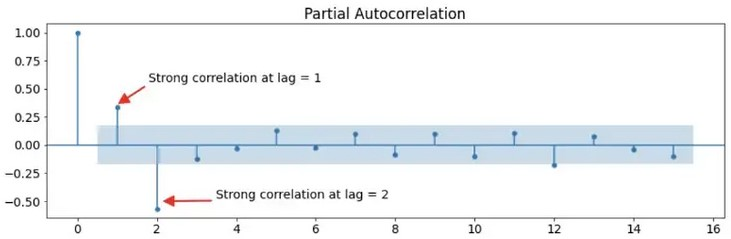
\includegraphics[width=1\textwidth]{images/PACF_AR(2).jpg}
        \subcaption{\ac{PACF} of \ac{AR}$(2)$}   
        \label{fig:PACF_AR}
    \end{subfigure}
    \begin{subfigure}[t]{0.5\textwidth}
        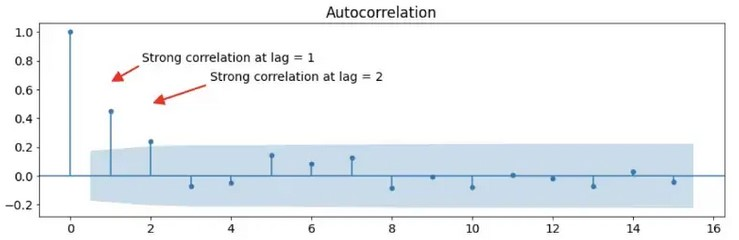
\includegraphics[width=1\textwidth]{images/ACF_MA(2).jpg}
        \subcaption{\acs{ACF} of \ac{MA}$(2)$}
        \label{fig:ACF_AR}
    \end{subfigure}
    \caption{Plots of two time series from \cite{P_ACF}. Values outside of the blue confidence interval are considered non-zero and thus, statistically relevant. \autoref{fig:PACF_AR}, \autoref{fig:ACF_AR} indicate respectively $p=2$, $q=2$.}
\end{figure}

A \ac{MA} model assumes the value $X_t$ for time unit $t$ is based on the correlated lagged (previous) errors $\omega_{t-j}, 0 < j \le q$, the mean of the series $\mu$ and an error term $\omega_t \sim  N(0, \sigma^2)$ as stated in \eqref{eq:MA}.
%
\begin{ceqn}
    \begin{equation}
    \label{eq:MA}
        X_t = \mu + \sum_{j=1}^q \theta_j \omega_{t-j} + \omega_t
    \end{equation}
\end{ceqn}
%
The calculation of the coefficients $\theta = (\theta_1, ..., \theta_q)$ is analogue to \ac{AR}.
This model assumes that the observations are located around the mean $\mu$, hence that the time series is stationary ($\mu, \sigma$ constant over time).
Thus, \eqref{eq:MA} without $\omega_t$ predicts $X_t$ based on the mean of the series and taking certain lagged errors $\omega_{t-j}$ into account. 
The error $\omega_t$ is added to calculate the real observation.
The number of statistically relevant lagged errors $\omega_{t-j}$ is indicated by $q$, which is calculated using an \acfi{ACF}.
\ac{ACF} is graphically visualised in \autoref{fig:ACF_AR} by plotting the autocorrelation value on the y-axis and the lags ($t - i, 0 \le i$) on the x-axis. It is important to note that a data point displayed is the indirect and direct correlation of $X_t$ and $X_ {t-i}$ calculated using \autoref{eq:pearson_corr}. Lagged observations considered statistically relevant are identified as stated above.
%
\begin{ceqn}
    \begin{equation}
    \label{eq:ARMA}
        X_t = c + \omega_t + \sum_{i=1}^p \phi_i X_{t-i} + \sum_{j=1}^q \theta_j \omega_{t-j} 
    \end{equation}
\end{ceqn}
%
The \acfi{ARMA} model in \eqref{eq:ARMA} is a combination of the \ac{AR} \eqref{eq:AR} and the \ac{MA} \eqref{eq:MA} models. The components are computed as stated above. However, the assumption of the \ac{MA} model, a time series is stationary, is not always true. Therefore, an \ac{ARIMA}($p, d, q$) model is constructed using the \ac{ARMA} model and the possibility of applying differencing of degree $d$ to data points to make them stationary (if necessary).

The Box-Jenkins method is used to tune the \ac{ARIMA} model. 
Firstly, the \acfi{ADF} test verifies if the time series is stationary.
The \ac{ADF} test rejects either hypothesis $H_0: \phi_i = 1 \Rightarrow \text{not stationary}$ or $H_1: \phi_i < 1 \Rightarrow \text{stationary}$.
Secondly, $p, q$ are configured as stated above.
Then, the training phase estimates coefficients $\phi, \theta$ as stated above.

\begin{figure}[http]
    \begin{center}
      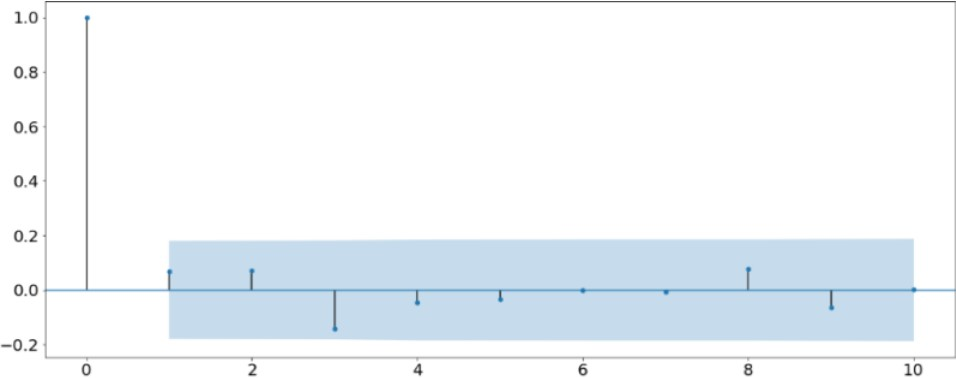
\includegraphics[scale=0.25]{images/ARIMA_correlogram_white_noise.jpg}
      \caption{Correlogram of residuals from \cite{fd_ARIMA}. A correlogram is the visualisation of the correlation of $X_t$ with lagged observations of $X$. Since none of the lagged residuals is considered statistically relevant, the model selected is optimal.}
      \label{fig:ARIMA_corr}
    \end{center}
\end{figure}

Lastly, the model is evaluated. For an ideal model, the error is normally distributed with mean $\mu$ of 0, constant variance $\sigma$ and the residuals are stationary (no temporal structure) as illustrated in \autoref{fig:ARIMA_corr}.

In order to detect fraudulent credit card transactions, the time series is split into a training (preferably only containing legitimate transactions) and testing set. 
The \ac{ARIMA} model is trained applying the Box-Jenkins method to the training set.
%
\begin{ceqn}
    \begin{equation}
    \label{eq:z-score}
        z = \frac{x-\mu}{\sigma}
    \end{equation}
\end{ceqn}
%
The fraudulent transactions of the testing set are identified by comparing the Z-score from \eqref{eq:z-score}, $x$ being the difference between predicted and actual \texttt{daily count of transactions}, $\mu, \sigma$ being the mean and variance based on the errors in predictions of the training set, with a certain threshold. A Z-score higher than the threshold corresponds to a fraudulent day.
